\section{分析手法}

\subsection{使用ツール}

本分析ではCytoscape 3.10.4を使用した．
Cytoscapeはネットワーク可視化・分析のためのオープンソースソフトウェアであり，
生物学的ネットワークの解析を主目的として開発されたが，
社会ネットワーク分析にも広く利用されている．

\subsection{分析指標}

ネットワーク指標の算出には，Cytoscapeの「Tools → Analyze Network」機能を使用した．
この機能により，各ノードに対して次数，媒介中心性，近接中心性などの指標が自動的に計算され，
ノードテーブルに属性として追加される．
算出された指標値は，可視化スタイルのマッピングに使用できる．

以下の指標を算出し，ネットワーク構造を分析した：

\begin{itemize}
  \item \textbf{次数（Degree）}: ノード$v$に接続するエッジの総数．有向グラフでは入次数と出次数の合計となる：
  \[
    \text{Degree}(v) = \text{InDegree}(v) + \text{OutDegree}(v)
  \]
  友人の多さを示す．
  \item \textbf{入次数（InDegree）}: 他者から向けられたエッジ数．人気度を示す．
  \item \textbf{出次数（OutDegree）}: 自分から向けたエッジ数．積極性を示す．
  \item \textbf{媒介中心性（Betweenness Centrality）}: ノード$v$の媒介中心性$C_B(v)$は以下の式で計算される：
  \[
    C_B(v) = \sum_{s \neq v \neq t} \frac{\sigma_{st}(v)}{\sigma_{st}}
  \]
  ここで$\sigma_{st}$はノード$s$から$t$への最短経路の総数，$\sigma_{st}(v)$はそのうち$v$を経由する経路数である．この値が高いほど，異なるノード間を繋ぐ橋渡し役として重要であることを示す．
  \item \textbf{近接中心性（Closeness Centrality）}: ノード$v$から他の全ノードへの最短経路長の平均の逆数：
  \[
    C_C(v) = \frac{n-1}{\sum_{u \neq v} d(v, u)}
  \]
  ここで$d(v,u)$は$v$から$u$への最短経路長，$n$はノード数である．情報へのアクセス容易性を示す．
  \item \textbf{クラスタ係数（Clustering Coefficient）}: ノード$v$の隣接ノード間の接続密度：
  \[
    C(v) = \frac{2 \cdot e_v}{k_v(k_v - 1)}
  \]
  ここで$k_v$は$v$の隣接ノード数，$e_v$は隣接ノード間のエッジ数である．グループの結束度を示す．
\end{itemize}

\section{分析結果}

\subsection{入次数中心性分析}

図\ref{fig:degree_size}に，入次数（他者から友人として選ばれた数）に基づくノードサイズの可視化を示す．
ノードサイズが大きいほど多くの人から友人として選ばれていることを表す．

\begin{figure}[htbp]
\centering
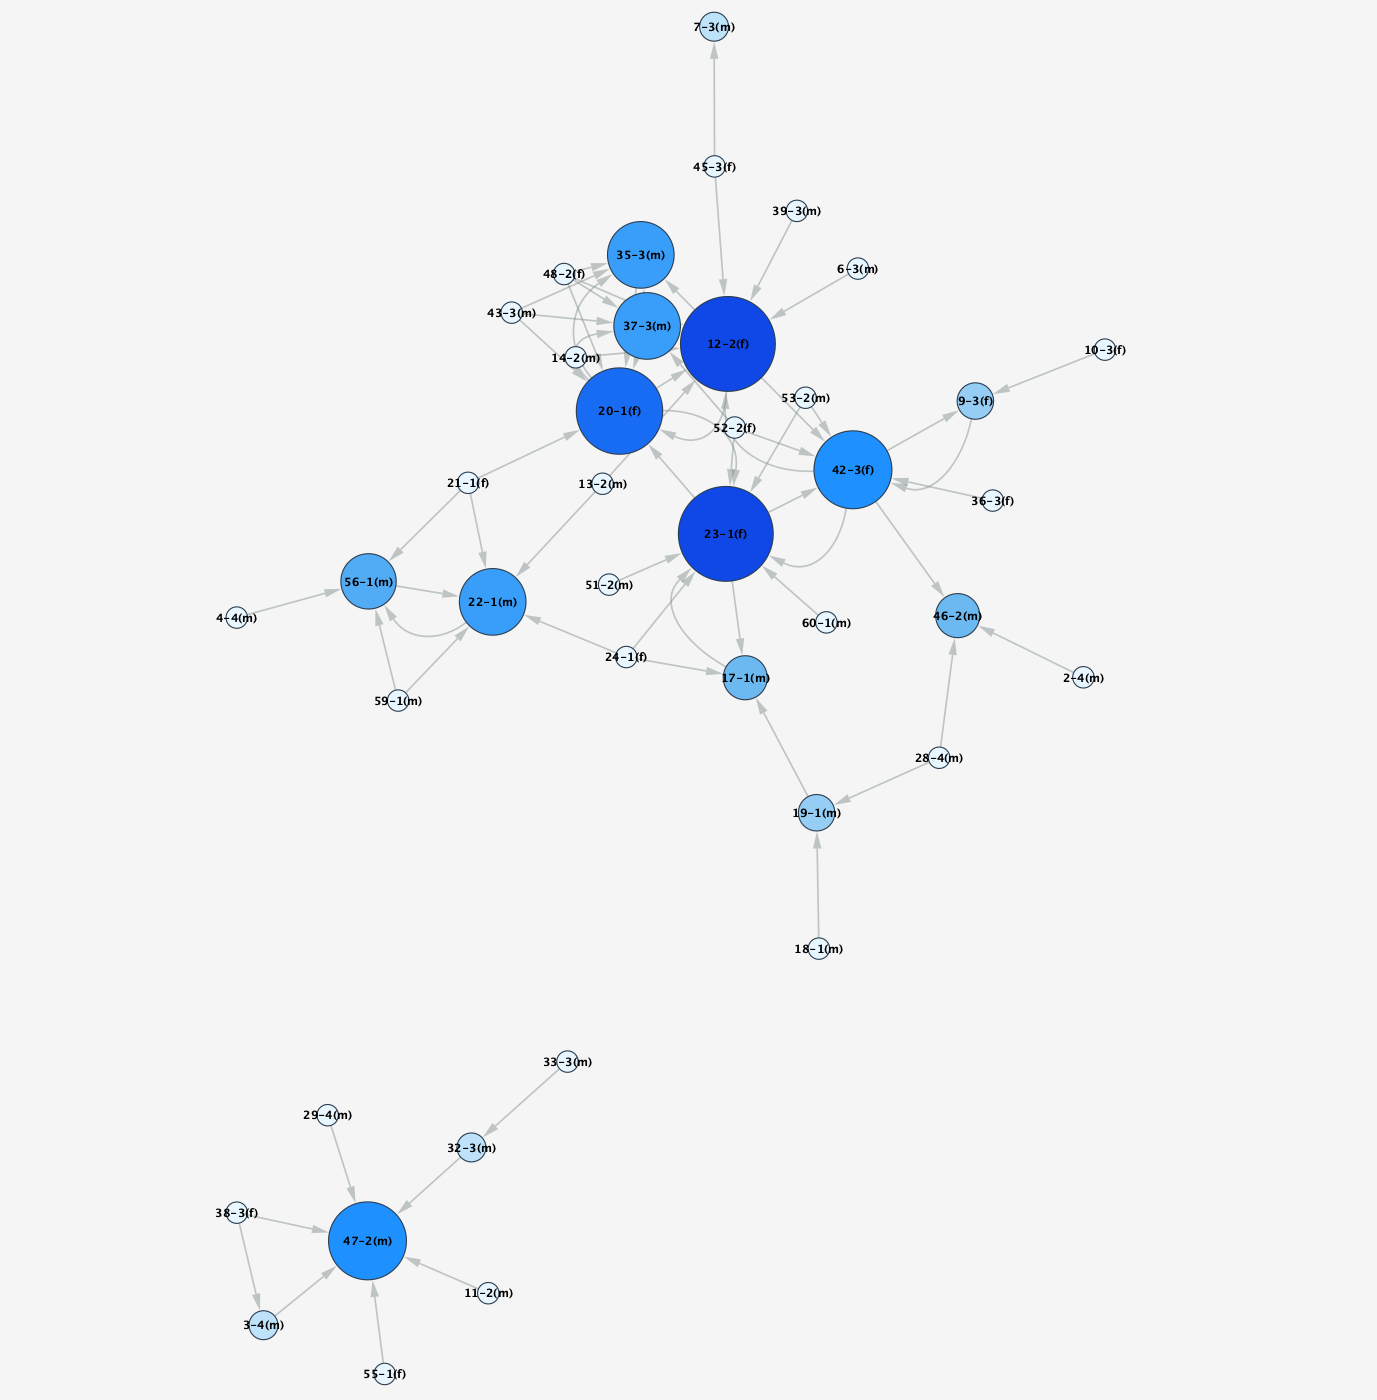
\includegraphics[width=0.95\linewidth]{fig/degree_size.png}
\caption{入次数中心性による可視化（Afterネットワーク）．ノードサイズと色は入次数に比例する（大きく濃いほど入次数が高い）．}
\label{fig:degree_size}
\end{figure}

Afterネットワークにおいて，特に入次数が高いノードとして
12-2(f)，20-1(f)，23-1(f)などが確認された．
これらのノードはネットワークにおいて人気が高く，ハブとして機能している．

\subsection{媒介中心性分析}

図\ref{fig:betweenness}に，媒介中心性に基づく可視化を示す．
可視化では，媒介中心性の値に応じてノードサイズと色を連続的にマッピングした．
具体的には，媒介中心性が0.0のノードは小さく薄い色（淡黄色），
0.5以上のノードは大きく濃い色（紫）となるグラデーションを適用した．
これにより，異なるグループを繋ぐ橋渡し役として重要なノードが視覚的に識別できる．

\begin{figure}[htbp]
\centering
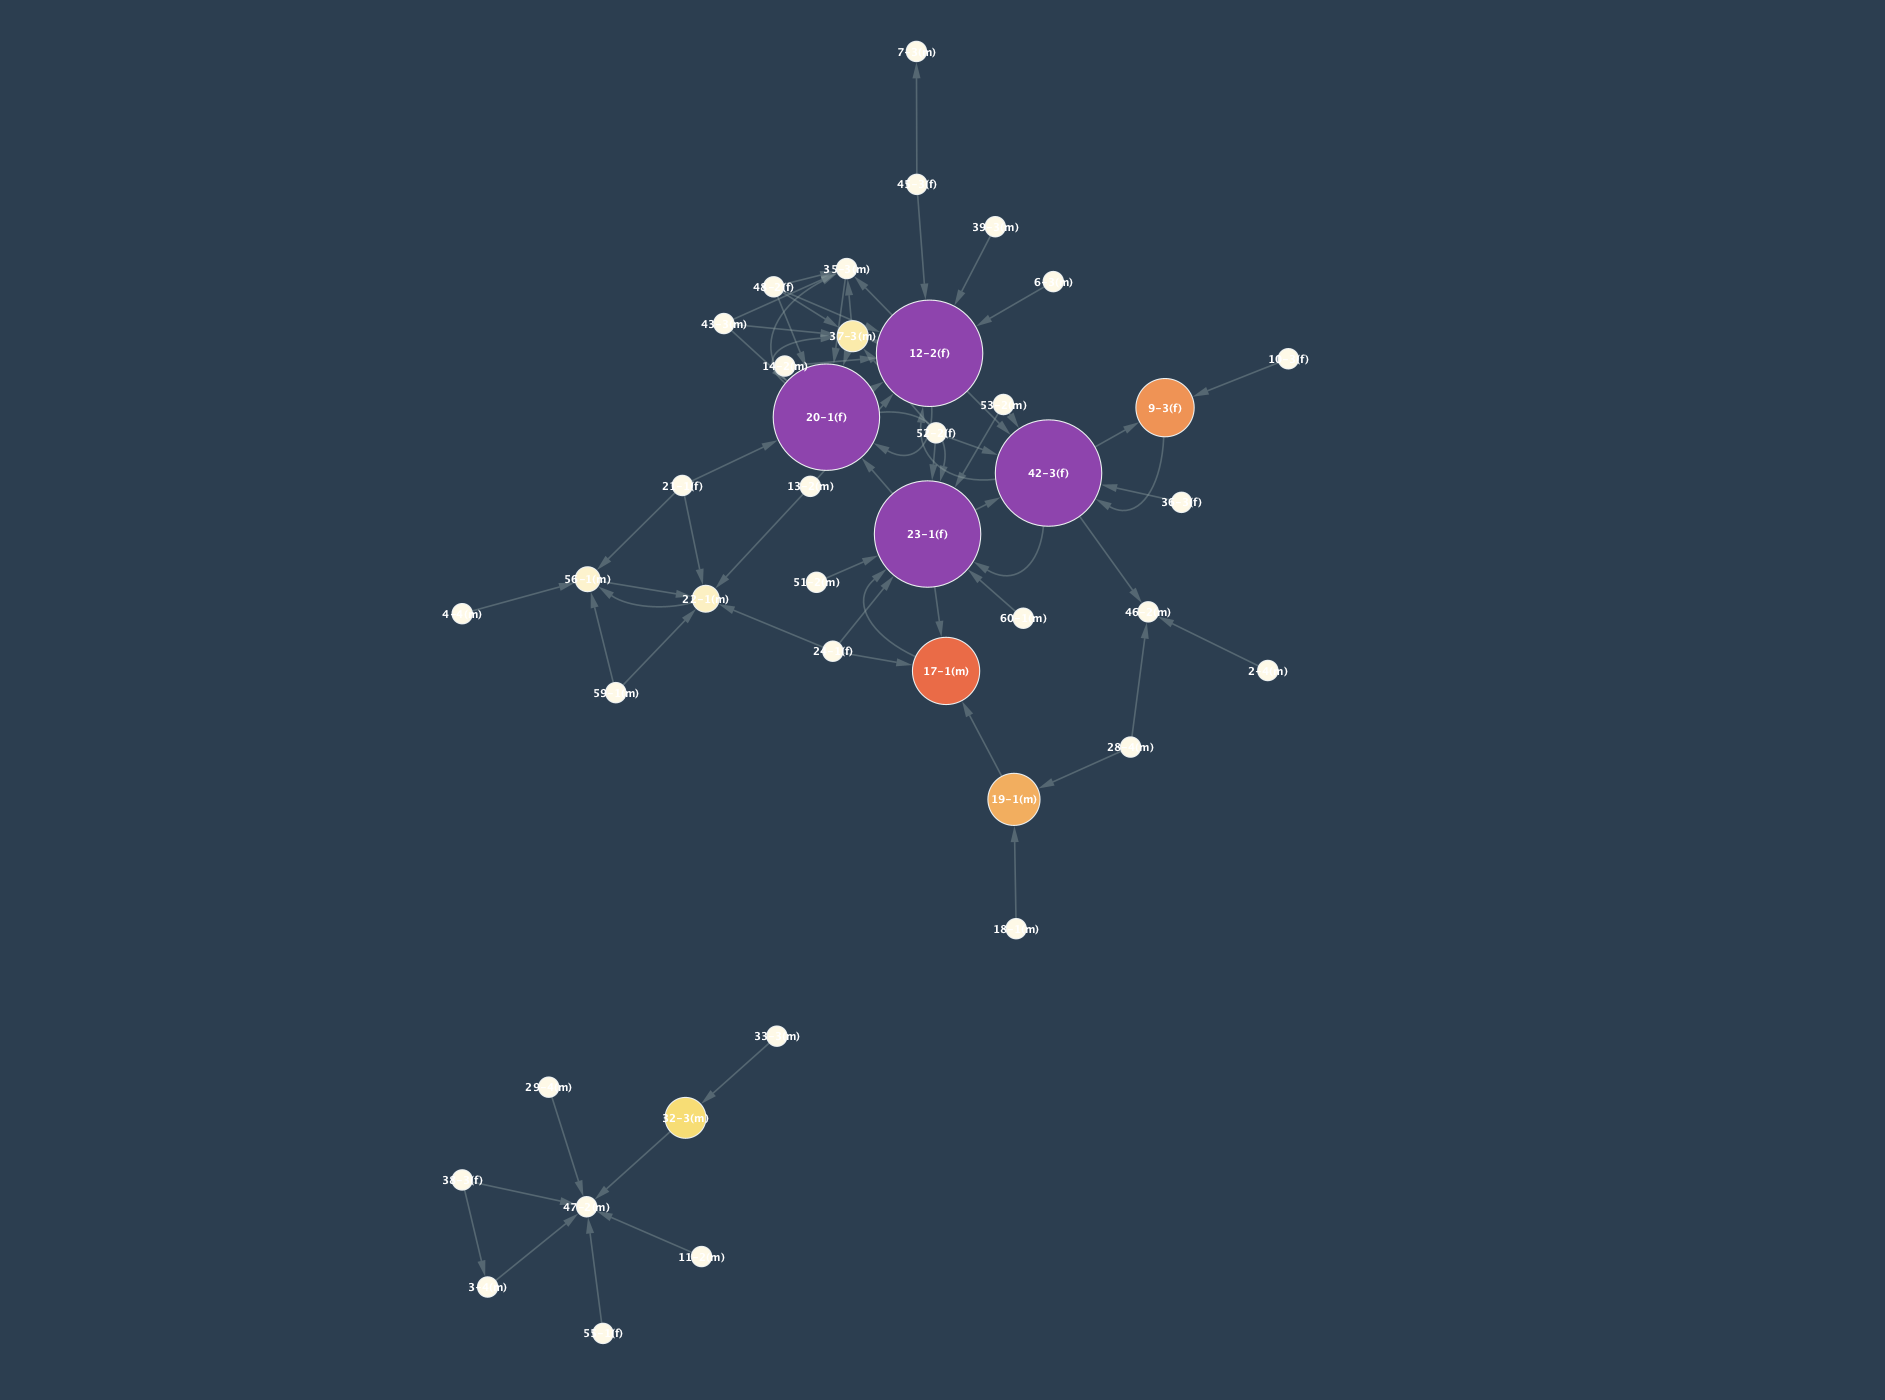
\includegraphics[width=0.95\linewidth]{fig/betweenness.png}
\caption{媒介中心性による可視化（Afterネットワーク）．ノードサイズと色は媒介中心性に比例する（大きく濃いほど橋渡し役として重要）．}
\label{fig:betweenness}
\end{figure}

媒介中心性が高いノードは，ネットワーク全体の情報伝達において重要な役割を果たす．
分析の結果，20-1(f)や23-1(f)が高い媒介中心性を示した．

\subsection{性別によるネットワークパターン}

図\ref{fig:network_before}および図\ref{fig:network_after}では，性別による色分け（ピンク：女性，青：男性）を適用している．

図\ref{fig:gender_edge}に，エッジの性別組み合わせによる色分けを示す．

\begin{figure}[htbp]
\centering
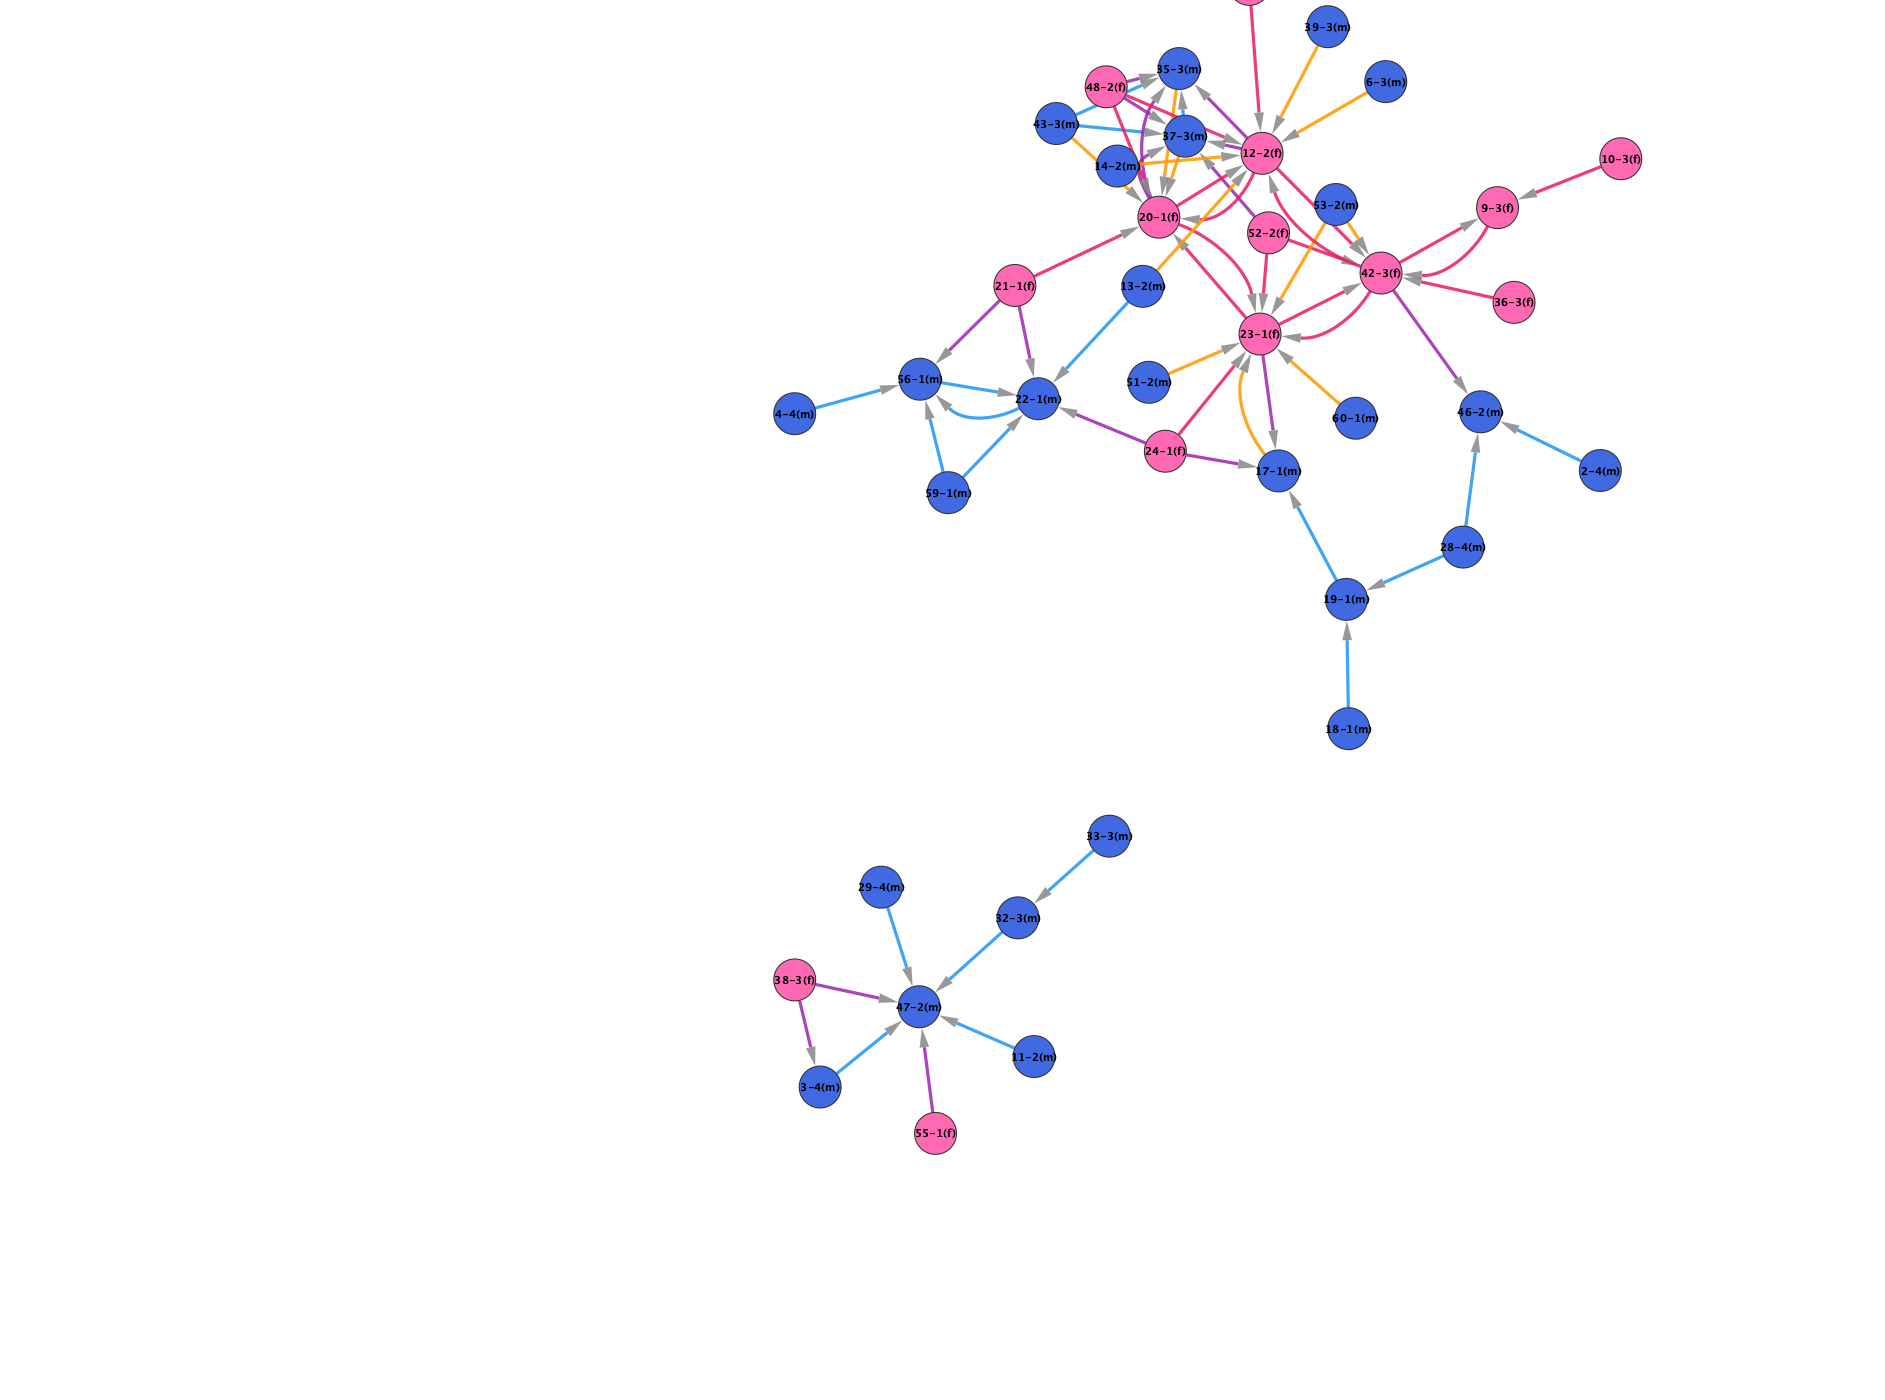
\includegraphics[width=0.95\linewidth]{fig/gender_edge.png}
\caption{エッジの性別組み合わせによる色分け（Afterネットワーク）．エッジ色：ピンク（女性→女性），紫（女性→男性），オレンジ（男性→女性），青（男性→男性）．ノード色：ピンク（女性），青（男性）．}
\label{fig:gender_edge}
\end{figure}

エッジの色分けは以下の通りである：
\begin{itemize}
  \item ピンク: 女性→女性
  \item 紫: 女性→男性
  \item オレンジ: 男性→女性
  \item 青: 男性→男性
\end{itemize}

\subsection{グループ間関係分析}

図\ref{fig:group_color}に，グループによる色分けを示す．
各ノードのグループ番号（ノードラベルの2番目の数字，例：「23-1(f)」のグループは1）に基づき，
離散的に色を割り当てた．

\begin{figure}[htbp]
\centering
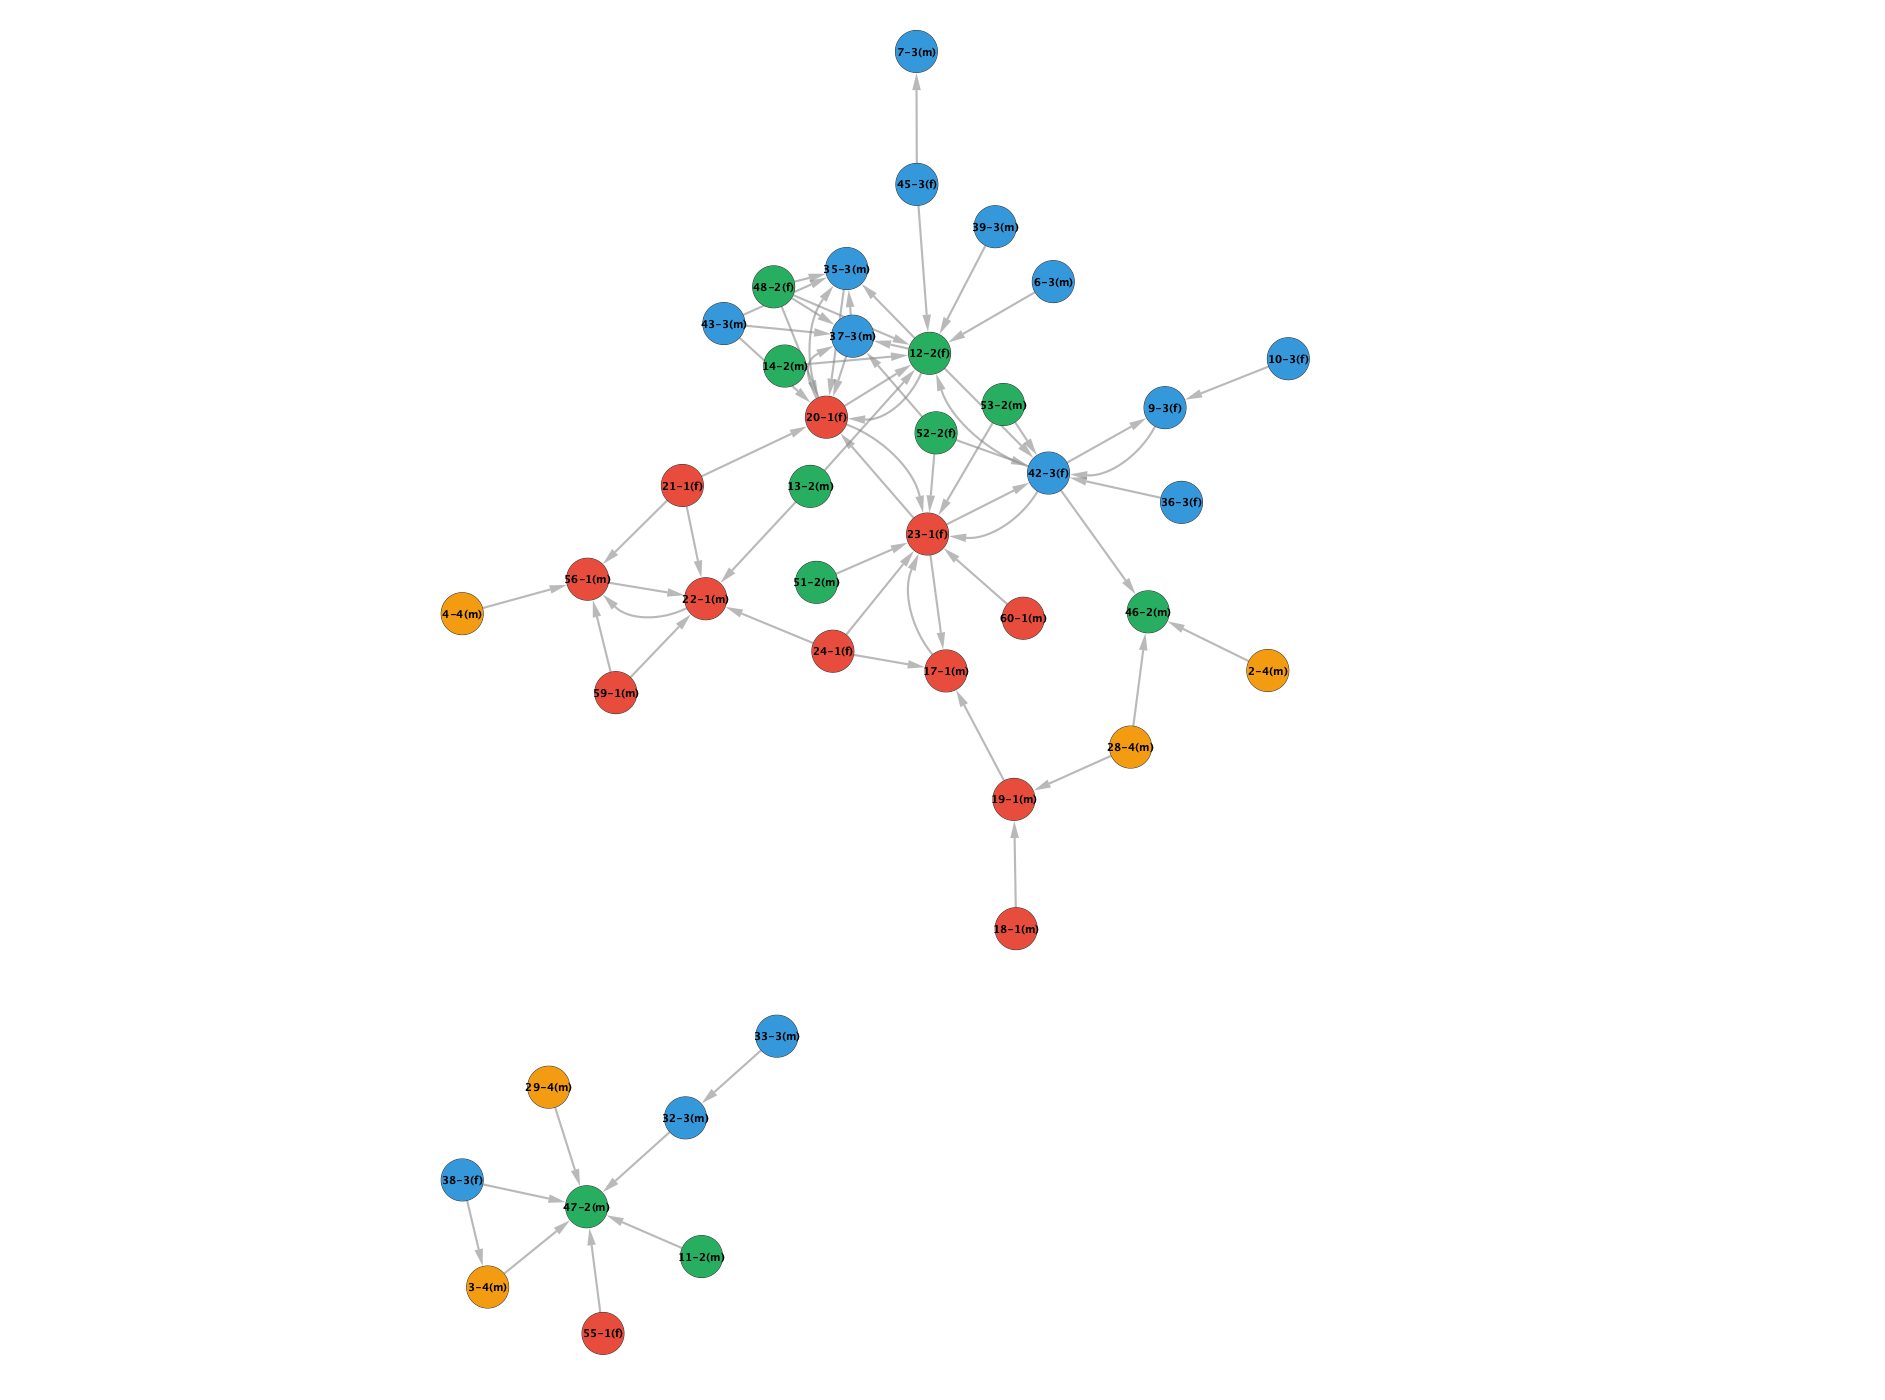
\includegraphics[width=0.95\linewidth]{fig/group_color.png}
\caption{グループによる色分け（Afterネットワーク）．ノード色はグループを示す（赤：グループ1，緑：グループ2，青：グループ3，オレンジ：グループ4）．}
\label{fig:group_color}
\end{figure}

グループ1（赤），グループ2（緑），グループ3（青），グループ4（オレンジ）で
ノードを色分けした結果，グループ間にも友人関係が形成されていることが確認できた．
特にグループ1と2の間，グループ2と3の間に多くのエッジが観察された．
